\chapter{Basics of Reinforcement learning}

\begin{comment}
    What is reinforcement learning in words, no equation or algorithms.
    
    How it is different from other types of machine learning.
     - Supervised learning
     - Unsupervised learning
    
    The different elements in reinforcement learning.
     - markov decision process
     - exploration
     - exploitation
     - agent   
     - environment
      • state
      • action
      • reward
     - policy
      • e-greedy
     - value
     - reward
      • different approaches to define rewards
        · continuos rewards
        · reward only at goal
        · negative reward while still alive
     - optional model
     - on/off policy
     - etc

    Very simple example of reinforcement learning.
     - tic-tac-toe
     - 1D travel (1D grid world, wins if it reaches one end, dies if it reaches the other.)
     - quad grid nav (this is more complex that what I would like to have here)
\end{comment}


% Introduction
\acrfull{rl} is a method of machine learning different from other machine learning methods such as supervised learning which uses a set of labeled examples from a knowledgeable supervisor, and unsupervised learning which is typically used to find hidden patterns in unlabeled data. In \gls{rl} the learner is not told what action to take to achieve its goal, but instead it maps situations and actions by trying them out and discovering the most valuable. It does this by not only looking at the reward it received by it's latest action, but it also takes into account any future rewards it could receive in the future by taking that action.

\section{Finite Marcov Decision Process}

\begin{comment}

  process that gives mathematical framework that can be used to describe problems where learners learn from their actions to reach a goal.

  Two main parts
  agent: decides, interacts with environment and learns
  environment everything else

  They constantly interact.
  agent decides and does action -> environment changes state and gives reward to agent -> agent learns.

  The probability of going from state to state only depends on the current state and the action, past states have no influence.


\end{comment}


A \acrfull{mdp} is a stochastic process that provides a mathematical framework used to describe problems where a learner learns from its actions to achieve an end goal. This framework is used in many areas, such as robotics, economics, manufacturing and in the case of this report, \acrlong{rl}. 

% source: intro and wiki
The two main components of an \gls{mdp} are the agent, which makes decisions, interacts with its environment and learns. And the environment which consists of everything else. The two are constantly interacting with each other, the agent will perform an action which changes the state of the environment and the environment responds by giving it a reward. The goal of the agent is to maximize the reward it receives from the environment.

This happens in a sequence of discrete time steps. At the beginning of each time step the environment is at a certain state $s$. The agent then decides based on its policy $\pi$ which action $a$ to take, this in turn changes the environment to the new state $s'$ and the environment then gives the agent a certain reward $r$. In order for it to be a \gls{mdp} this transition and the reward must satisfy the Marcov property, which means it needs to be memoryless and thus the environment's behavior must be independent of its past states. In other words, the probability of the environment to go from state $s$ to $s'$ and the reward $r$ it gives back to the agent, must only be dependent on the initial state $s$ and action $a$.

\section{Elements of Reinforcement Learning}

% intro
The main goal when solving an \gls{mdp} problem is to find a policy $\pi$ that defines the action $\pi\left(s\right)$ the agent will take in order to maximize the sum of rewards it receives. It characterizes the way in which the agent will behave at a given time by mapping the agents perceived state of the environment to the actions taken in those states. This policy may be as simple as a table or consist of several Neural Networks. The policy is the core of the agent in that it alone defines the behavior of the agent.

On each time step the environment will send the agent a reward. The goal of the agent is to maximize this reward in the long run. Thus this reward is used to tell the agent which states are good or bad. If the agent receives a low reward for a certain action it can change the policy so it takes a different action in the future.

The reward signal tells the agent what the immediate effects of its action are. However, its goal is to maximize the cumulative sum of rewards it receives over time, and thus in order for it to receive higher rewards in the future, it might be necessary for the agent to take actions that yield lower rewards with the promise that it will receive higher rewards later. So the value is an indication of the reward the agent can expect to receive in the future by taking a certain action, and thus it is the main parameter used in the decision making process. 

By defining the action taken during step $t$ as $A_t$, and its corresponding reward as $R_t$ we can define the true value of an arbitrary action $a$ as:

\begin{equation}
  q_*\left (a \right )\dot{=}\ \mathbb{E}\left[R_t\ |\ A_t=a \right ]
\end{equation}

If $q_*(a)$ was known, then the solution would be trivial. Just select the action with the highest value. So it's assumed that the action values are not known, but are instead estimated from the rewards the agent receives. The estimated value of action $a$ at time $t$ is known as $Q_t(a)$, thus $Q_t(a)$ needs to be as close to $q_*(a)$ as possible.

Finally some \gls{rl} agents make use of a model for planning. This allows these agents to choose actions based on possible future situations before actually being experienced.


\section{k-armed bandit problem}
K-armed bandit problems will be used as examples in the following sections. These are simple learning problems where the agent is given the option to take $k$ different action's. There is only one state and the episodes terminate after the agent has taken it's action. Furthermore the examples in this report use zero mean, unit variance normal distributions to select the true value $q_*(a)$ of the actions. The rewards given by the environment are then selected with $q_*(a)$ mean and unit variance normal distribution. Figure~\ref{fig:k_armed_bandit_vionlin} shows an example reward distribution for a 5-armed bandit.

\begin{figure}[ht]			
	\centering
	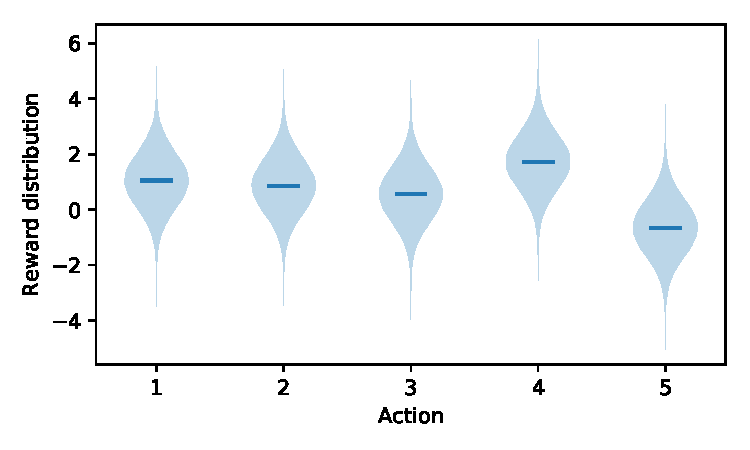
\includegraphics{figures/k_armed_bandit_violin}			
	\caption{Example reward distribution for a 5-armed bandit problem.}
	\label{fig:k_armed_bandit_vionlin}
\end{figure}


\section{\eps-greedy policies}
The main difference between \acrlong{rl} and other types of learning is that \gls{rl} uses training information that evaluates the actions taken by the agent instead of a set of correct actions. This means that in order to determine $Q_t(a)$ the agent needs to explore and try out as many actions as possible in order to find good behavior. To do this the agent can take random actions and learn from the rewards it gets back. This is called \emph{exploration}.

However, the main goal of the agent is to maximize the rewards it receives from the environment over time. To achieve this goal the agent can choose to take the greedy actions. These are the actions with the highest value in $Q_t(a)$. This process of choosing the greedy action is known as \emph{exploitation} since the agent is exploiting its knowledge to achieve its goal.

Unfortunately exploration and exploitation conflict with each other since in the former the agent wants to try out all possible actions, but only wants to perform a specific action if it's following a greedy policy. Thus a possible compromise is to use what is known as an \eps-greedy policy. In these policies, the agent will choose a random action \eps\ percentage of the time and the greedy action the rest of the time. This allows the agent to explore and try out new actions or old actions whose value might have changed, while also trying to achieve it's goal.

Since the agent is trying out new actions while following \eps-greedy policies, it is able to learn faster and more than if it was following a greedy policy. To demonstrate this 2000 10-armed bandit problems are run for 1000 episodes. The average reward of all bandits are stored after each episode. Figure ~\ref{fig:10_armed_bandit} shows the average reward and the percentage of agents that selected the optimal action for the greedy policy and two \eps-greedy policies ($\epsilon=0.1$ and $\epsilon=0.1$). A full explanation of the learning method used can be found in the section ????, but in short, the action value function $Q_t(a)$ is estimated by averaging the rewards received from the environment.

\begin{figure}[ht]			
	\centering
	
\includegraphics{figures/10_armed_bandit}			
	\caption{Average reward of 2000 10-armed bandit problems for 1000 episodes when following the greedy and two \eps-greedy policies.}
	\label{fig:10_armed_bandit}
\end{figure}

As it can be seen when using \eps-greedy policies the agents learn faster and are thus able to receive higher rewards sooner. On the other hand, while following the greedy policy, the agents will quickly choose the first action they find with a reward higher than the initial action value and then perform that action on all episodes. As a results many of the agents are not able to find the optimal policy.

